%https://www.overleaf.com/learn/latex/Beamer_Presentations:_A_Tutorial_for_Beginners_(Part_2)—Lists,_Columns,_Pictures,_Descriptions_and_Tables

%Usate il link sopra è una guida con tutti i comandi per le slidesss
\documentclass{beamer}

\usepackage{graphicx}           	% Allows including images
\usepackage{booktabs}         	  	% Allows the use of \toprule,
                                					% \midrule and \bottomrule in tables
\usepackage{tikz}               		% add background image

\usepackage{setspace}				%different line spacing can be achieved.




\title{WhereMI Bozza slide 2}
\subtitle{L'audioguida turistica del XXI secolo}
\author{
  Filippo Bartolucci
  \texttt{Matricola 0000838531}\\
  \and
  Umberto Case
  \texttt{Matricola 0000833051}\\
    \and
  Matteo Celani
  \texttt{Matricola 0000804303}\\
    \and
  Francesco Cerio
  \texttt{Matricola 0000832618}
 }
\institute{Università di Bologna}
\date{}

\setbeamertemplate{frametitle}[default][center]


\begin{document}

\begin{frame}
\titlepage
\end{frame}

\begin{frame}
\frametitle{Specifiche}
Where MI è un'app per trovare velocemente audioguide sul web. E' pensata per due tipi di utenti:
\begin{itemize}
  \item \textbf{Le guide}: postano gratuitamente video sul web
  \item \textbf{I turisti}: in cerca di consigli, cultura e svago
\end{itemize}
\vspace{0.2cm}
È composta da due web app:
\begin{itemize}
  \item \textbf{Il browser} permette al turista di trovare audio, video e testo dei luoghi d'interesse
  \item \textbf{L'editor} permette ad una guida di creare audio, video e testo associati ai luoghi e catalogarli
\end{itemize}
\vspace{0.2cm}
\centering Divisione Compiti
\vspace{0.2cm}
  \begin{columns}
    \begin{column}{.48\textwidth} % Left column and width
    Team Editor:
 \begin{itemize}
  \item Francesco Cerio
  \item Matteo Celani
\end{itemize}
    \end{column}
    \hfill
    \begin{column}{.48 \textwidth}
    Team Browser:
  \begin{itemize}
  \item Filippo Bartolucci
  \item Umberto Case
\end{itemize}
    \end{column}
  \end{columns}
\end{frame}

\begin{frame}
\frametitle{Diagrammi}
\begin{columns}
\column{0.5\textwidth}
	\centering 
	\begin{figure}[h]
	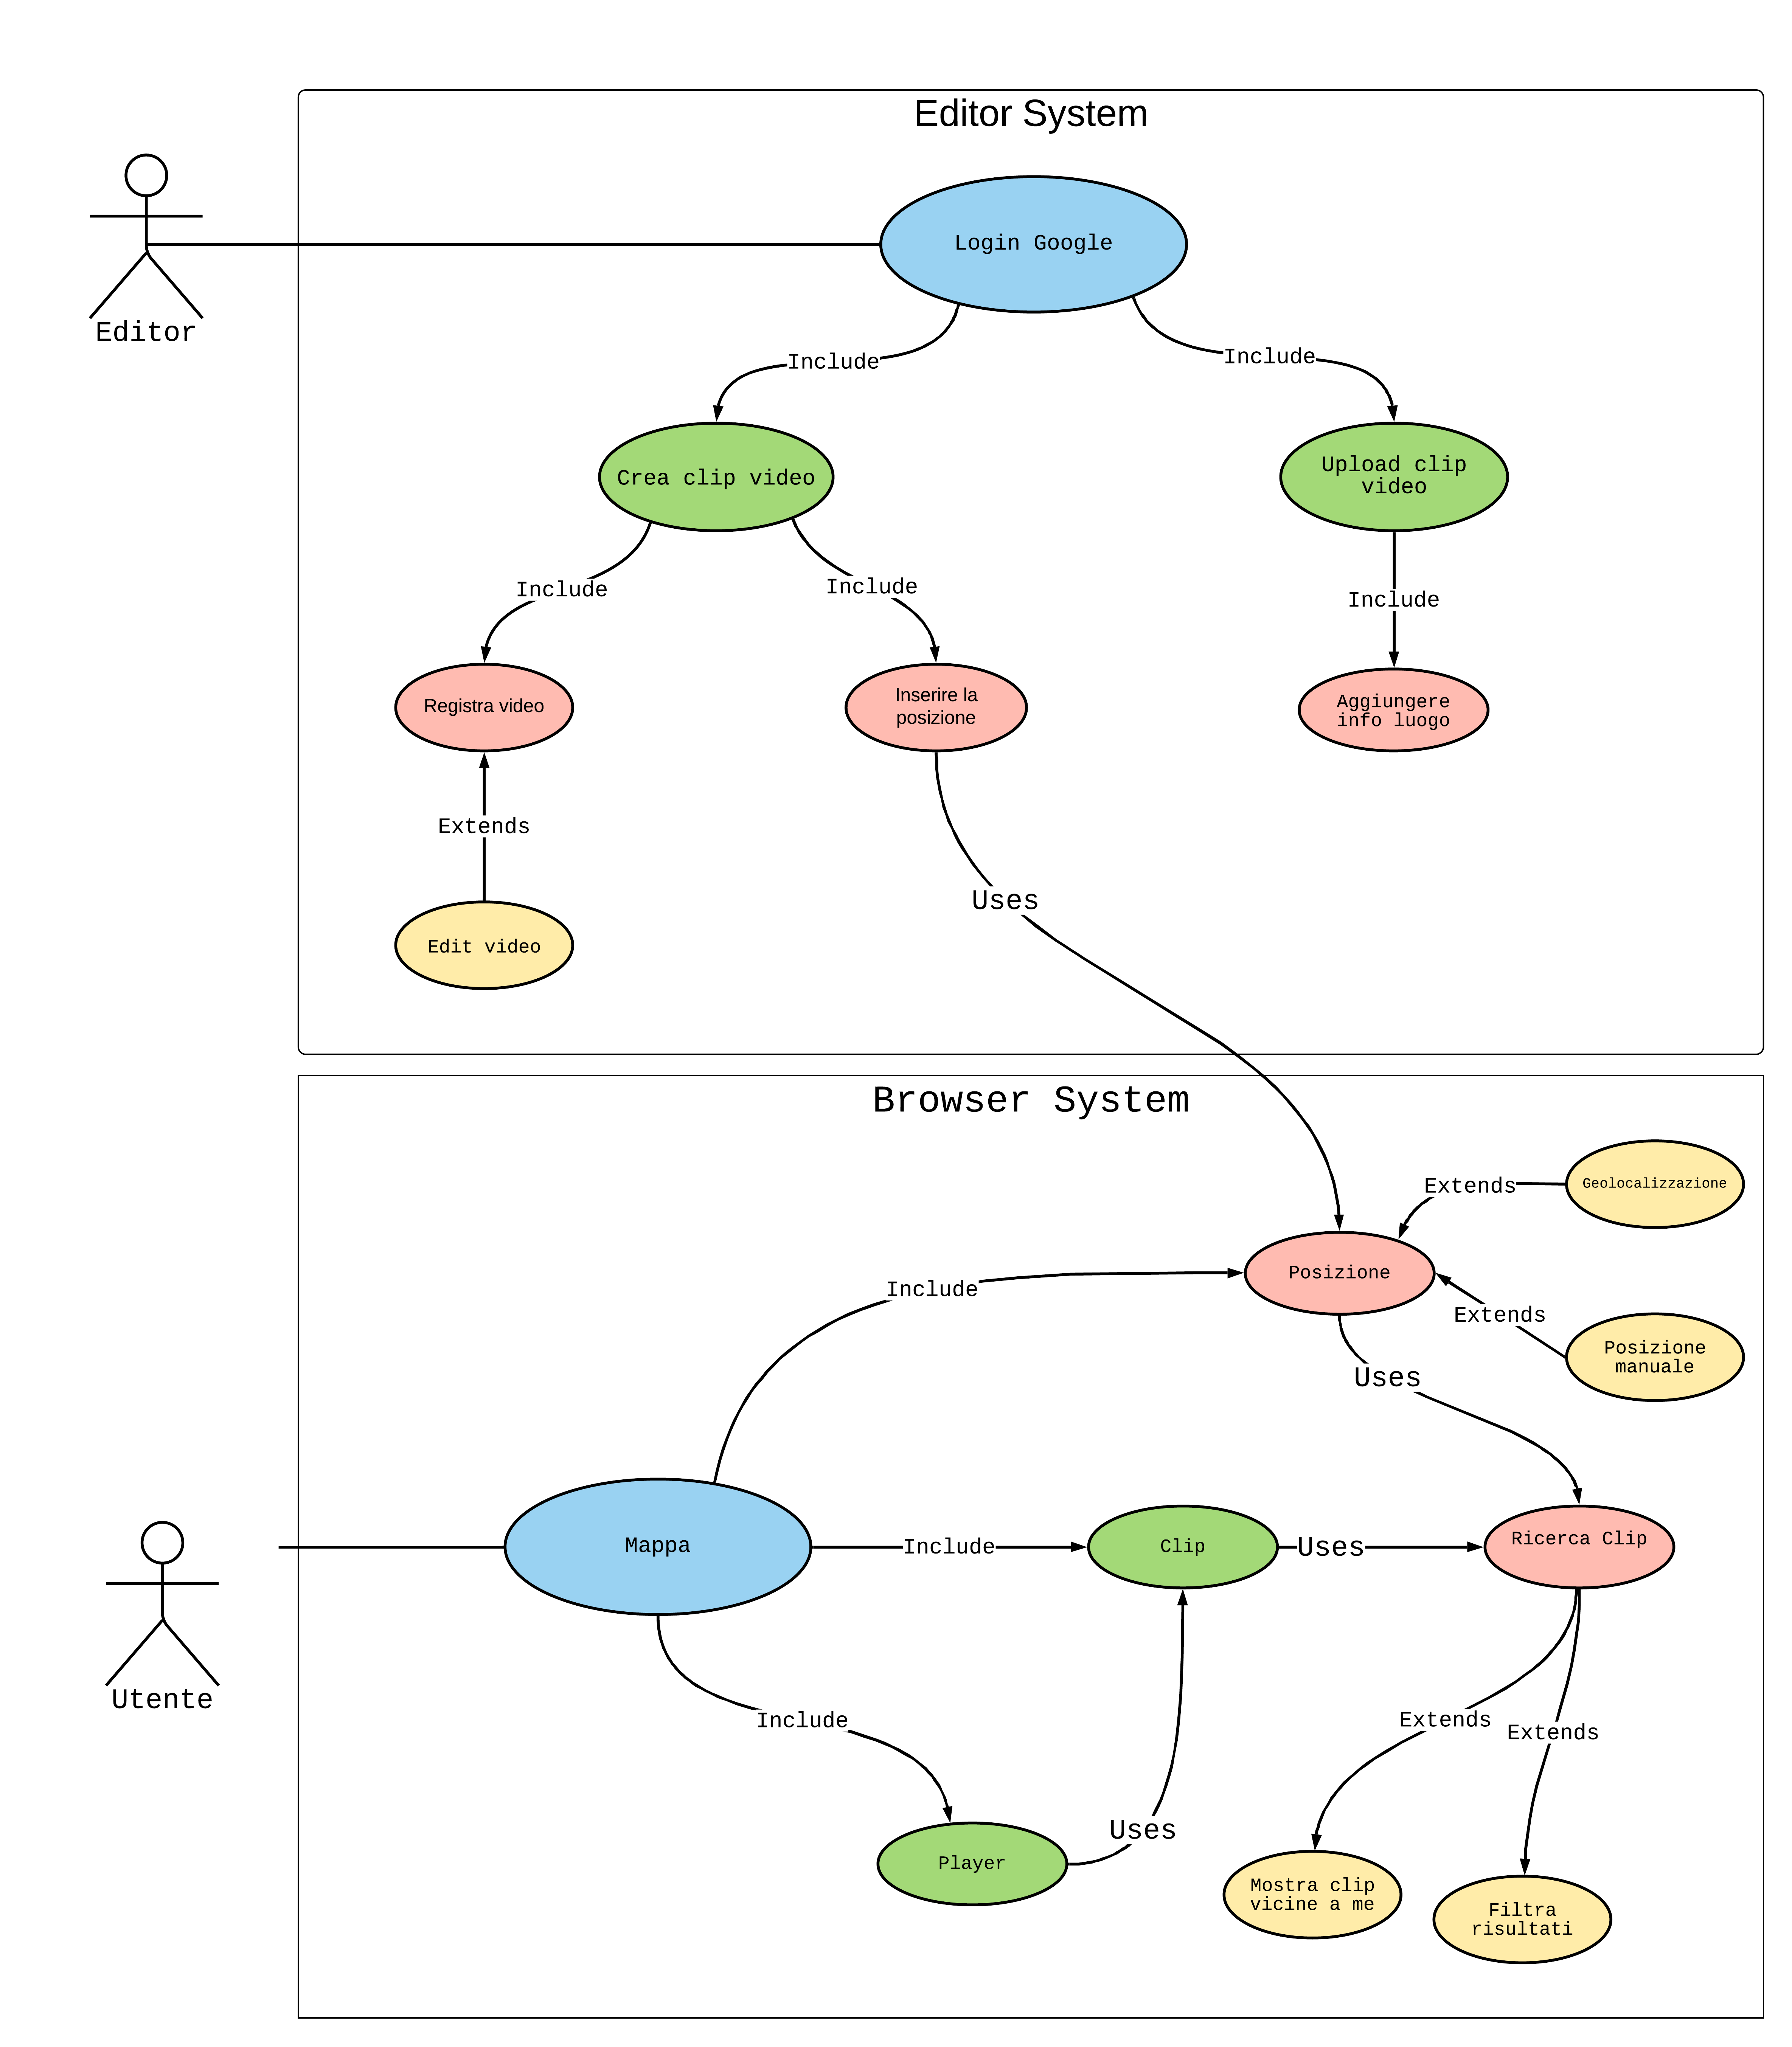
\includegraphics[width=5cm]{Images/UML/UML4.png}
	\vfill
	\caption{Casi d'uso}
	\end{figure}
	
\column{0.5\textwidth}
	\vspace{0.8cm}
	\centering 
	\begin{figure}[h]
	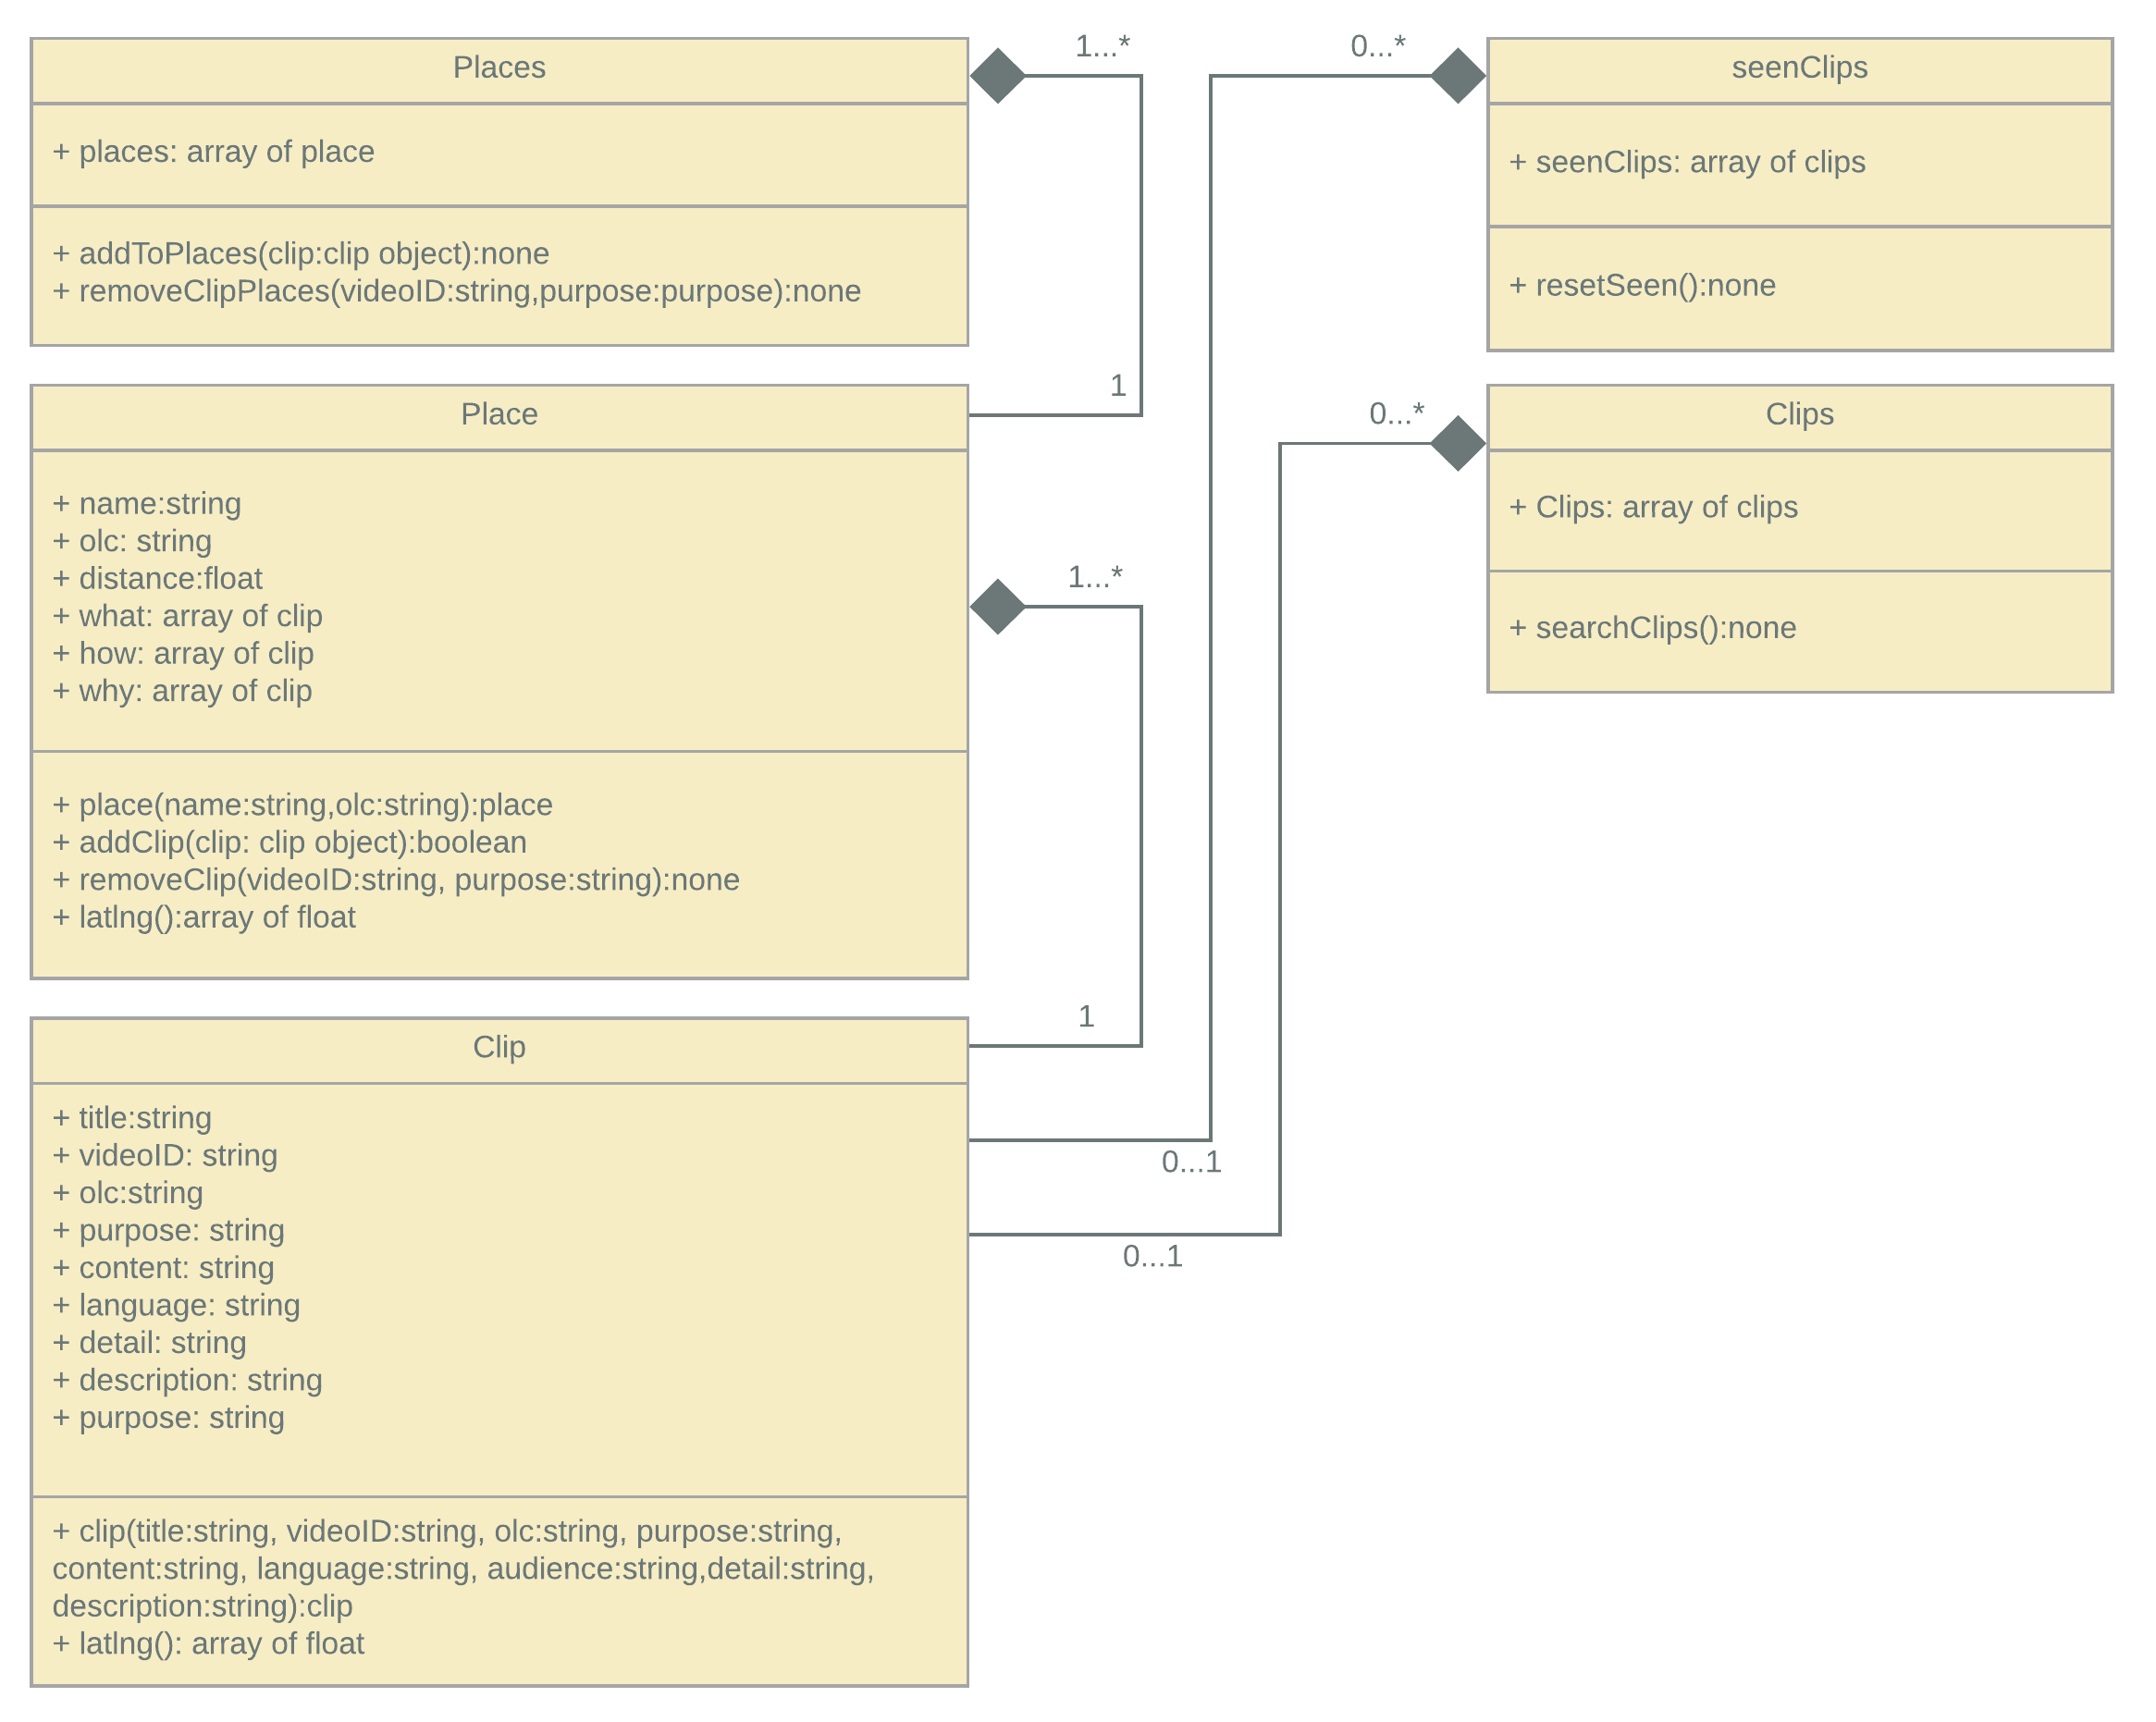
\includegraphics[width=5.5cm]{Images/diagramma_di_classe2.png}
	\caption{Diagramma di classe}
	\end{figure}
\end{columns}
\end{frame}

\begin{frame}
\frametitle{Organizzazione Taiga}
User Story
  \begin{itemize}
  	\item Divisione tra Editor e Browser
	\item Divide et Impera
	\item Utilizzo dei tag e punteggi UX/Design/Front/Back
	\item Utilizzo di commenti per mostrare i progressi nel loro sviluppo
  \end{itemize}
\vspace{5mm}
  Utilizzo del Kanban
    \begin{itemize}
	\item Monitoraggio dell'avanzamento del progetto
	\item Aggiornamento costante
  \end{itemize}
  \vspace{5mm}
  Nota: Non tutte le user story sono state effettivamente sviluppate
\end{frame}

\begin{frame}
\frametitle{Product Backlog}
\framesubtitle{Taiga}	   
  \begin{figure}[h]
  	\centering 
        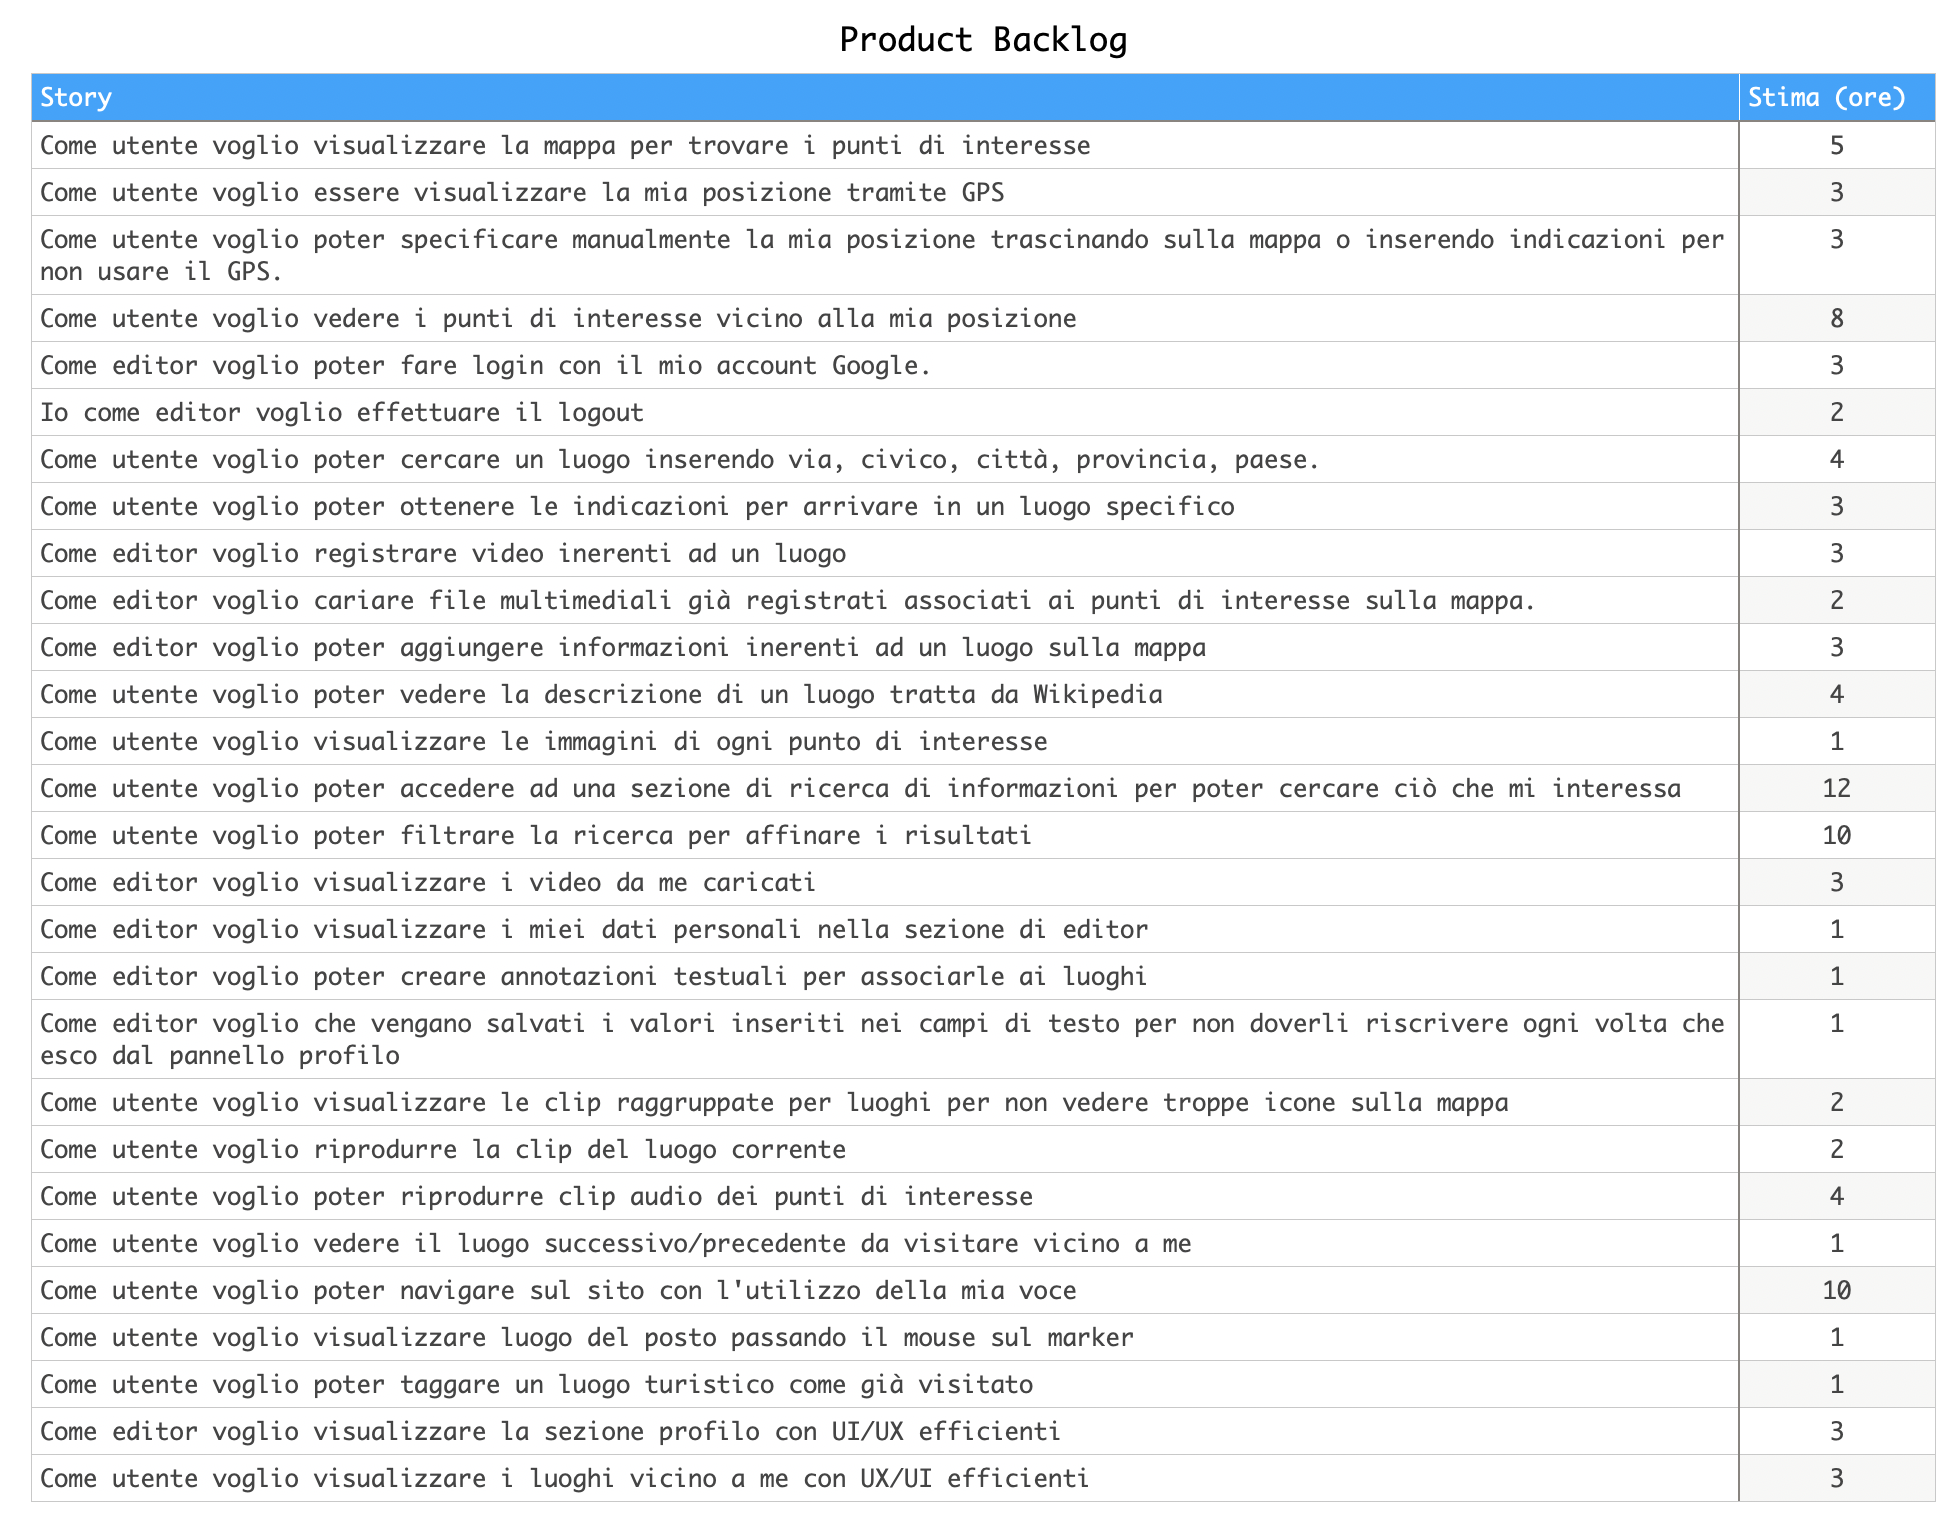
\includegraphics[width=9cm]{Images/Taiga/UserStory/backlog.png}
   \end{figure}
\end{frame}

\begin{frame}
\frametitle{Primo Sprint}
\framesubtitle{20/01/2020 - 03/02/2020}
\begin{columns}
\column{0.5\textwidth}
Obiettivo: 
  \begin{itemize}
	\item Mappa
	\item Login
	\item User Info
	\item Migliorare interfaccia Login
	\item Punti d'interesse vicino a me
	\item Css Clip
	\item Posizione Manuale
	\item Indicazioni
  \end{itemize}
\column{0.5\textwidth}
  \centering  
  \begin{figure}[h]
        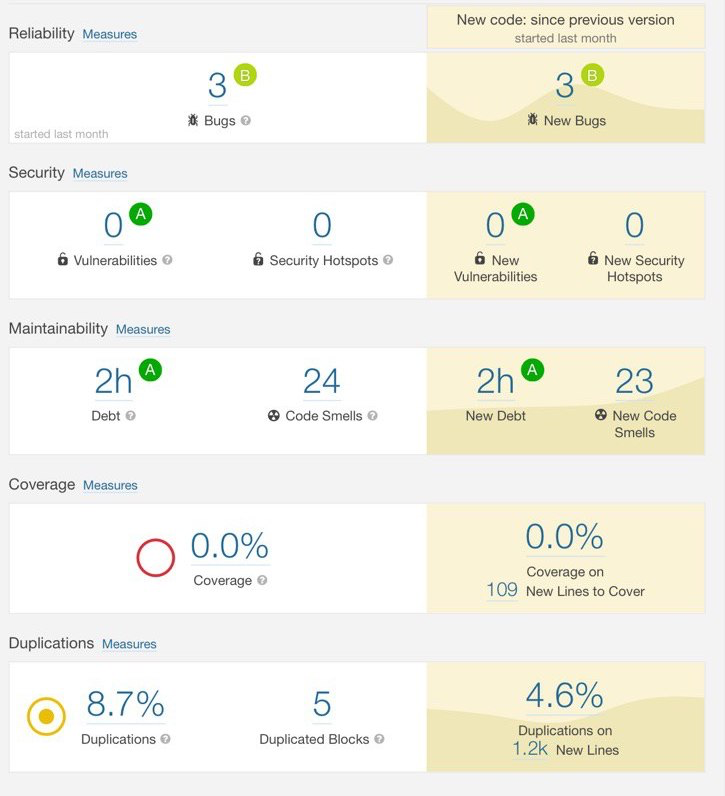
\includegraphics[width=5cm]{Images/SonarQube/primo-sprint.png}
        \caption{Analisi SonarQube}
   \end{figure}
\end{columns}
\end{frame}

\begin{frame}
\frametitle{Secondo Sprint}
\framesubtitle{03/02/2020 - 09/02/2020}
\begin{columns}
\column{0.5\textwidth}
Obiettivo:
  \begin{itemize}
	\item Creazione Contenuti
	\item Css vicino a me
	\item Popup on hover
	\item Clip luogo corrente
	\item Next/Prev
	\item Ricerca Contenuti
	\item Miglioro UI/UX
	\item Mostra contenuti
	\item Logout
  \end{itemize}
\column{0.5\textwidth}
	\begin{figure}[h]
        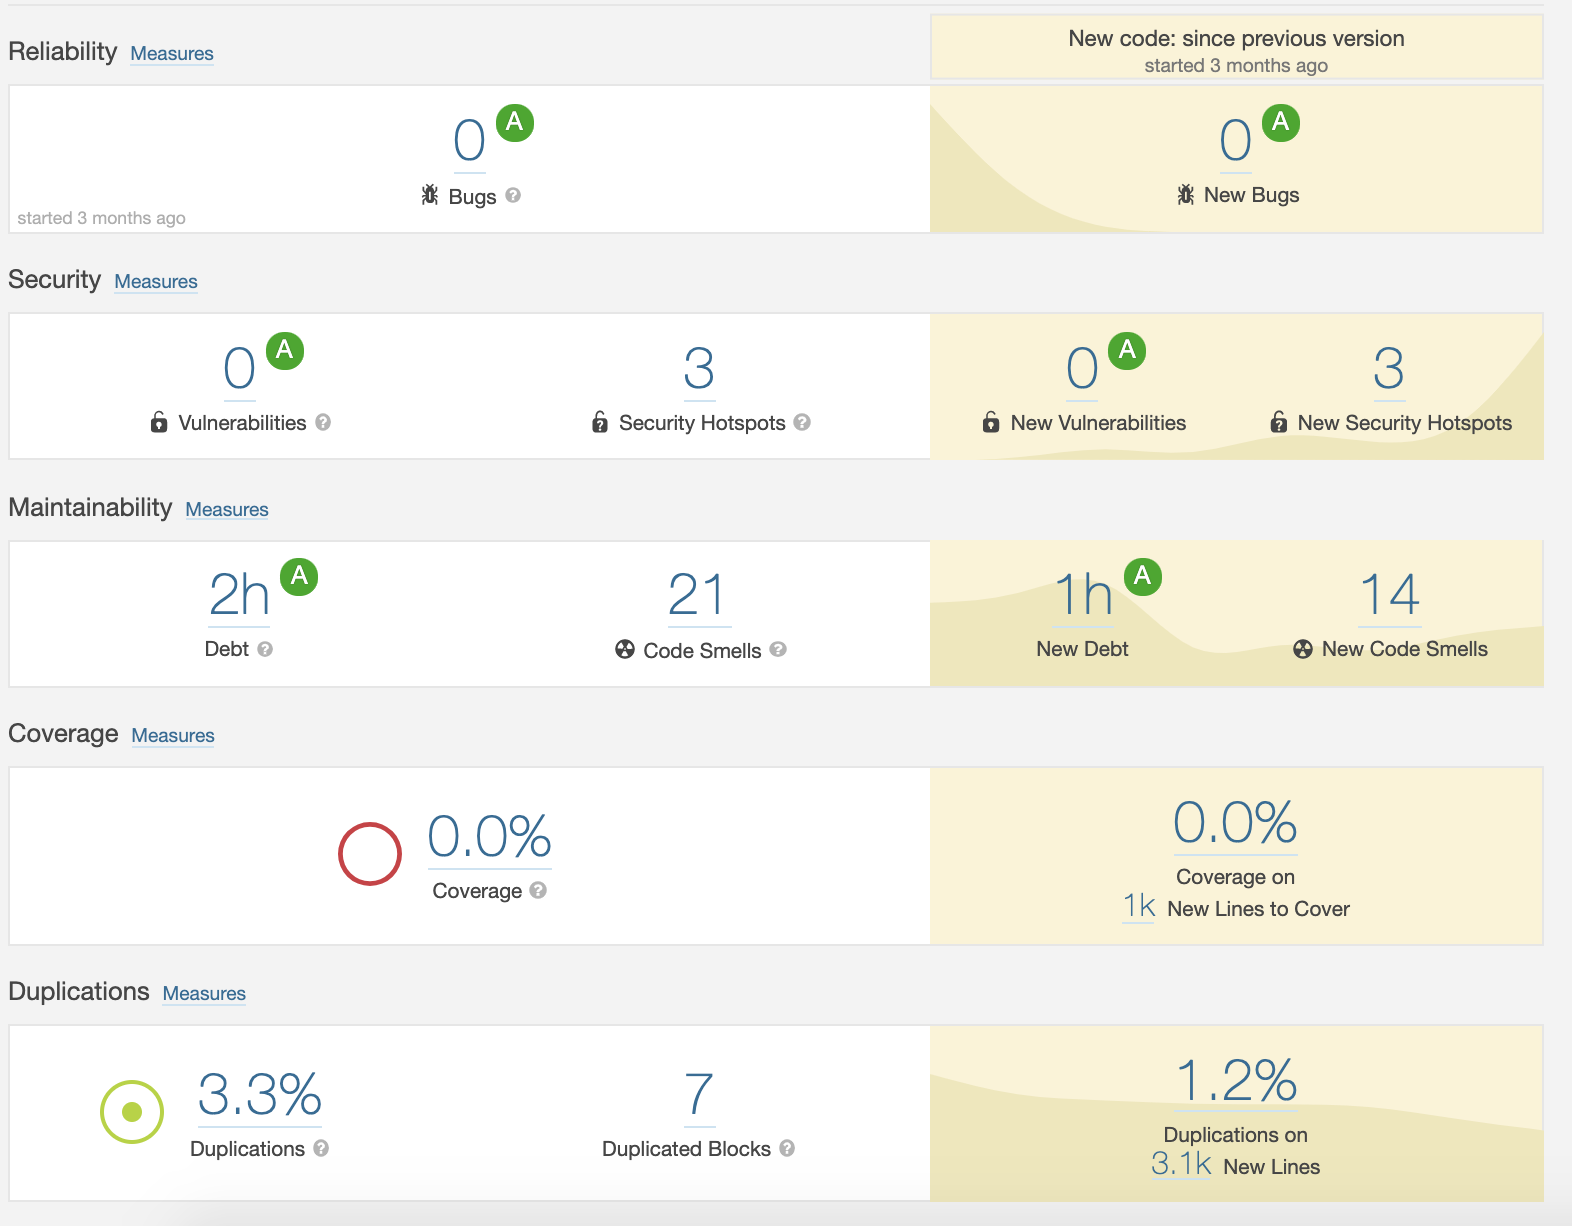
\includegraphics[width=5cm]{Images/SonarQube/terzo-sprint.png}
        \caption{Analisi SonarQube}
   \end{figure}
\end{columns}
\end{frame}

\begin{frame}
\frametitle{Terzo Sprint}
\framesubtitle{09/02/2020 - 13/02/2020}
\begin{columns}
\column{0.5\textwidth}
Obiettivo:
  \begin{itemize}
	\item Descrizione Wikipedia
	\item Feedback vocale
	\item Riproduci clip
	\item Filtro ricerca
	\item Creazione di annotazioni
	\item Ricerca immagini
	\item Aggiungere informazioni su un luogo
  \end{itemize}
\column{0.5\textwidth}
	\begin{figure}[h]
        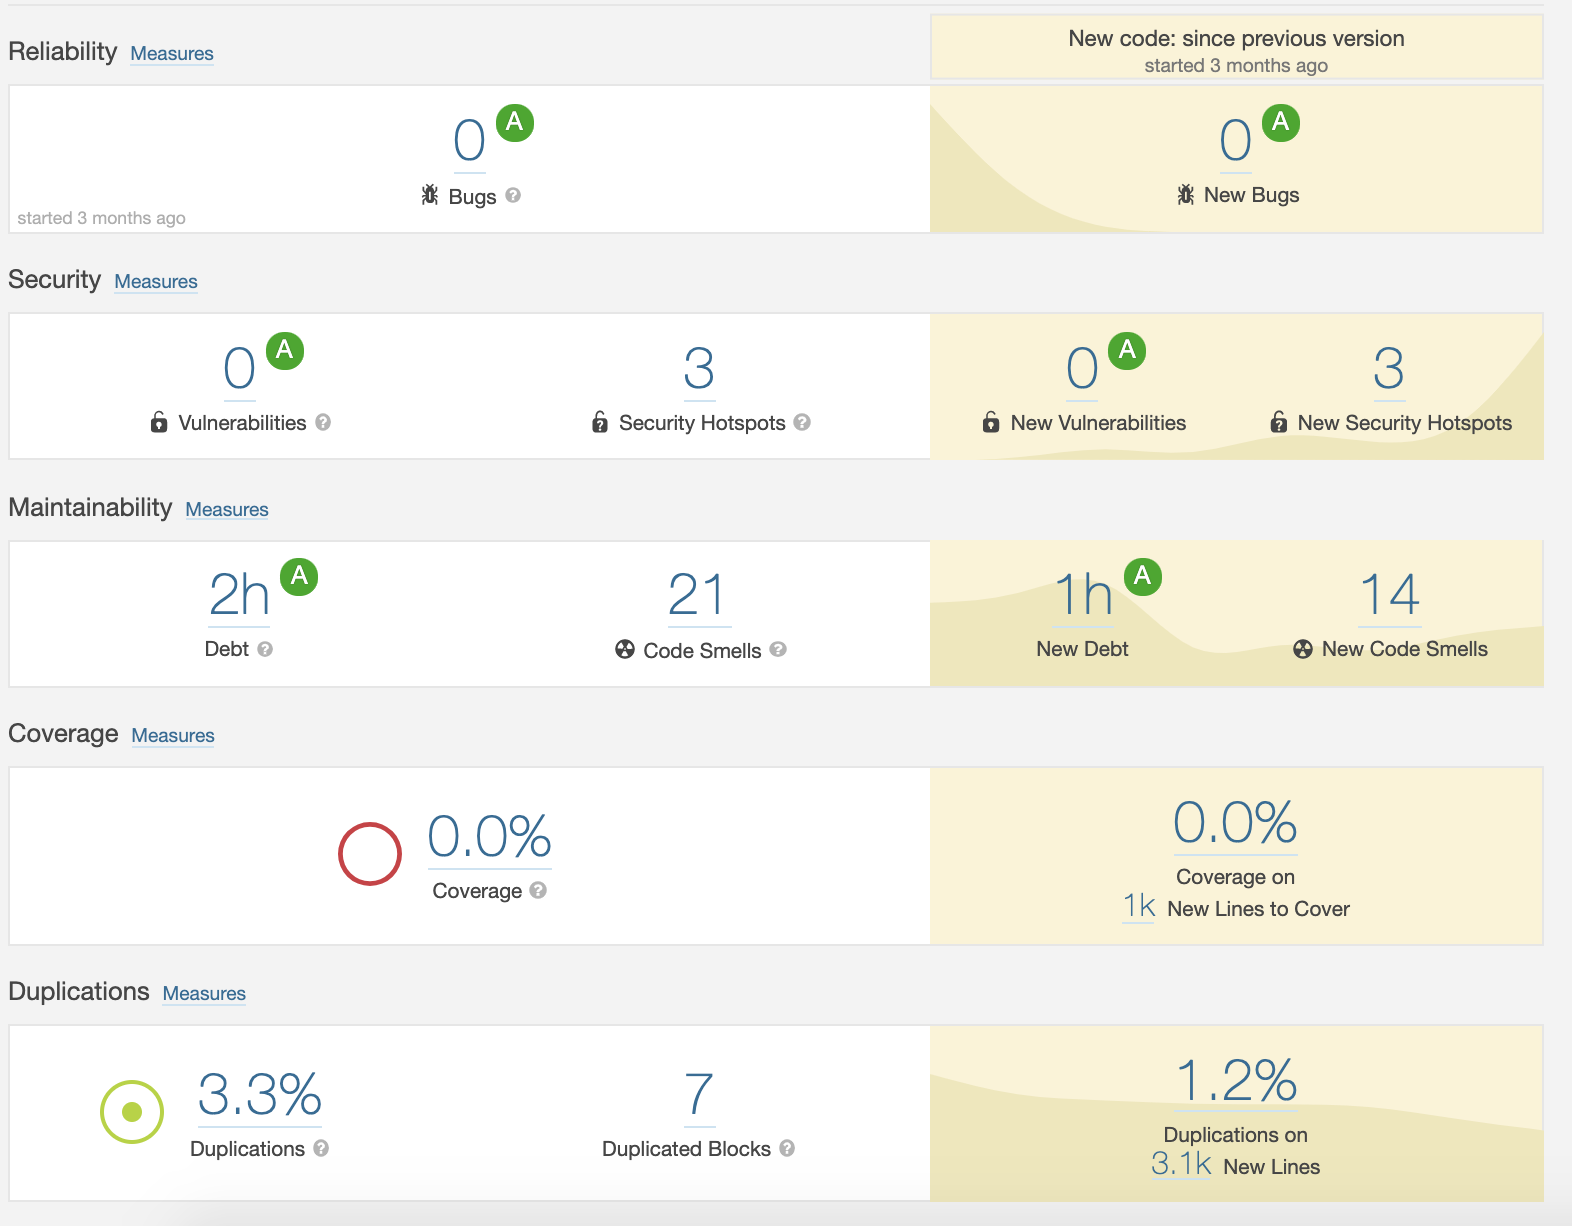
\includegraphics[width=5cm]{Images/SonarQube/terzo-sprint.png}
        \caption{Analisi SonarQube}
   \end{figure}
\end{columns}
\end{frame}

\begin{frame}
\frametitle{Quarto sprint}
\framesubtitle{20/02/2020 - 04/03/2020}
\begin{columns}
\column{0.5\textwidth}
Obiettivo:
  \begin{itemize}
	\item Controllo Vocale
	\item Ricerca Luogo
	\item Raggruppare le clip per luogo
	\item Luoghi già visitati
	\item Memorizzare campi editori
  \end{itemize}
\column{0.5\textwidth}
	\begin{figure}[h]
	\centering
        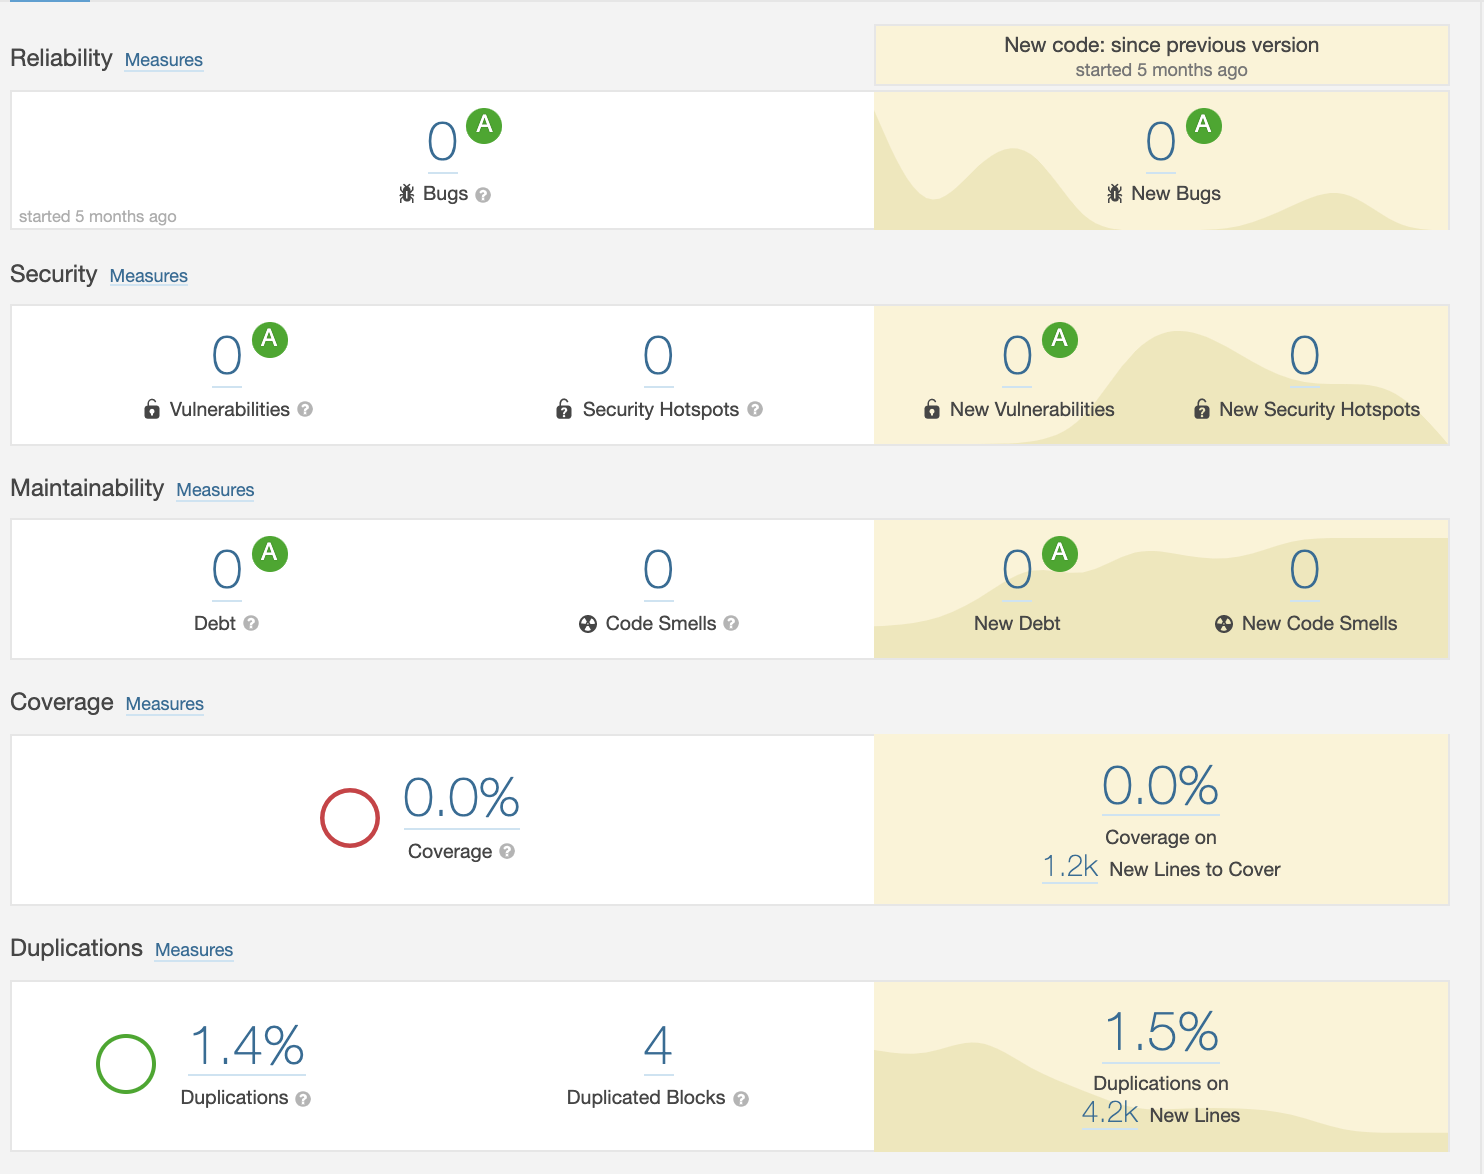
\includegraphics[width=5cm]{Images/SonarQube/ultimo-sprint.png}
        \caption{Analisi SonarQube}
   \end{figure}
\end{columns}
\end{frame}

%\begin{frame}
%\frametitle{Burndown}
%  \begin{enumerate}
%	\item Costruzione scheletro del sito
%	 	 \begin{enumerate}
%			\item WhereMI, VicinoMe, Cerca, Team,Profilo
%			\item Login, posizione, punti di interesse
%    		 \end{enumerate}
%	\item Sviluppo tecnologie e UI/UX
%		 \begin{enumerate}
%			\item Contenuti, ricerca, popup, logout
%			\item Next Prev, UI/UX, css
%     	 \end{enumerate}
%	\item Incrementato il numero di funzionalità
%		 \begin{enumerate}
%			\item Wikipedia, feedback, clip, filtri, annotazioni
%			\item Ricerca immagini, informazioni luogo
%      	\end{enumerate}
%	\item Implementazioni aggiuntive e correzioni finali
%		 \begin{enumerate}
%			\item Controllo vocale, raggruppato clip per luogo
%			\item Cookie
%      	\end{enumerate}
%  \end{enumerate}
%\end{frame}

\begin{frame}
\frametitle{Burndown}
\centering
\begin{tabular}{|c|c|c|c|c|c|c|c|c|}
\hline
					& Sprint 1.1	& Sprint 1.2	&Sprint 2.1	&Sprint 2.2	\\
Punteggio		& 247			& 285			& 380			& 251			\\
\hline
					&Sprint 3.1	&Sprint 3.2	&Sprint 4.1	&Sprint 4.1    \\
Punteggio 	& 138,5			& 136			& 168			& 78 			 	 \\
\hline
\end{tabular}
 \centering
        \begin{tabular}{c}
        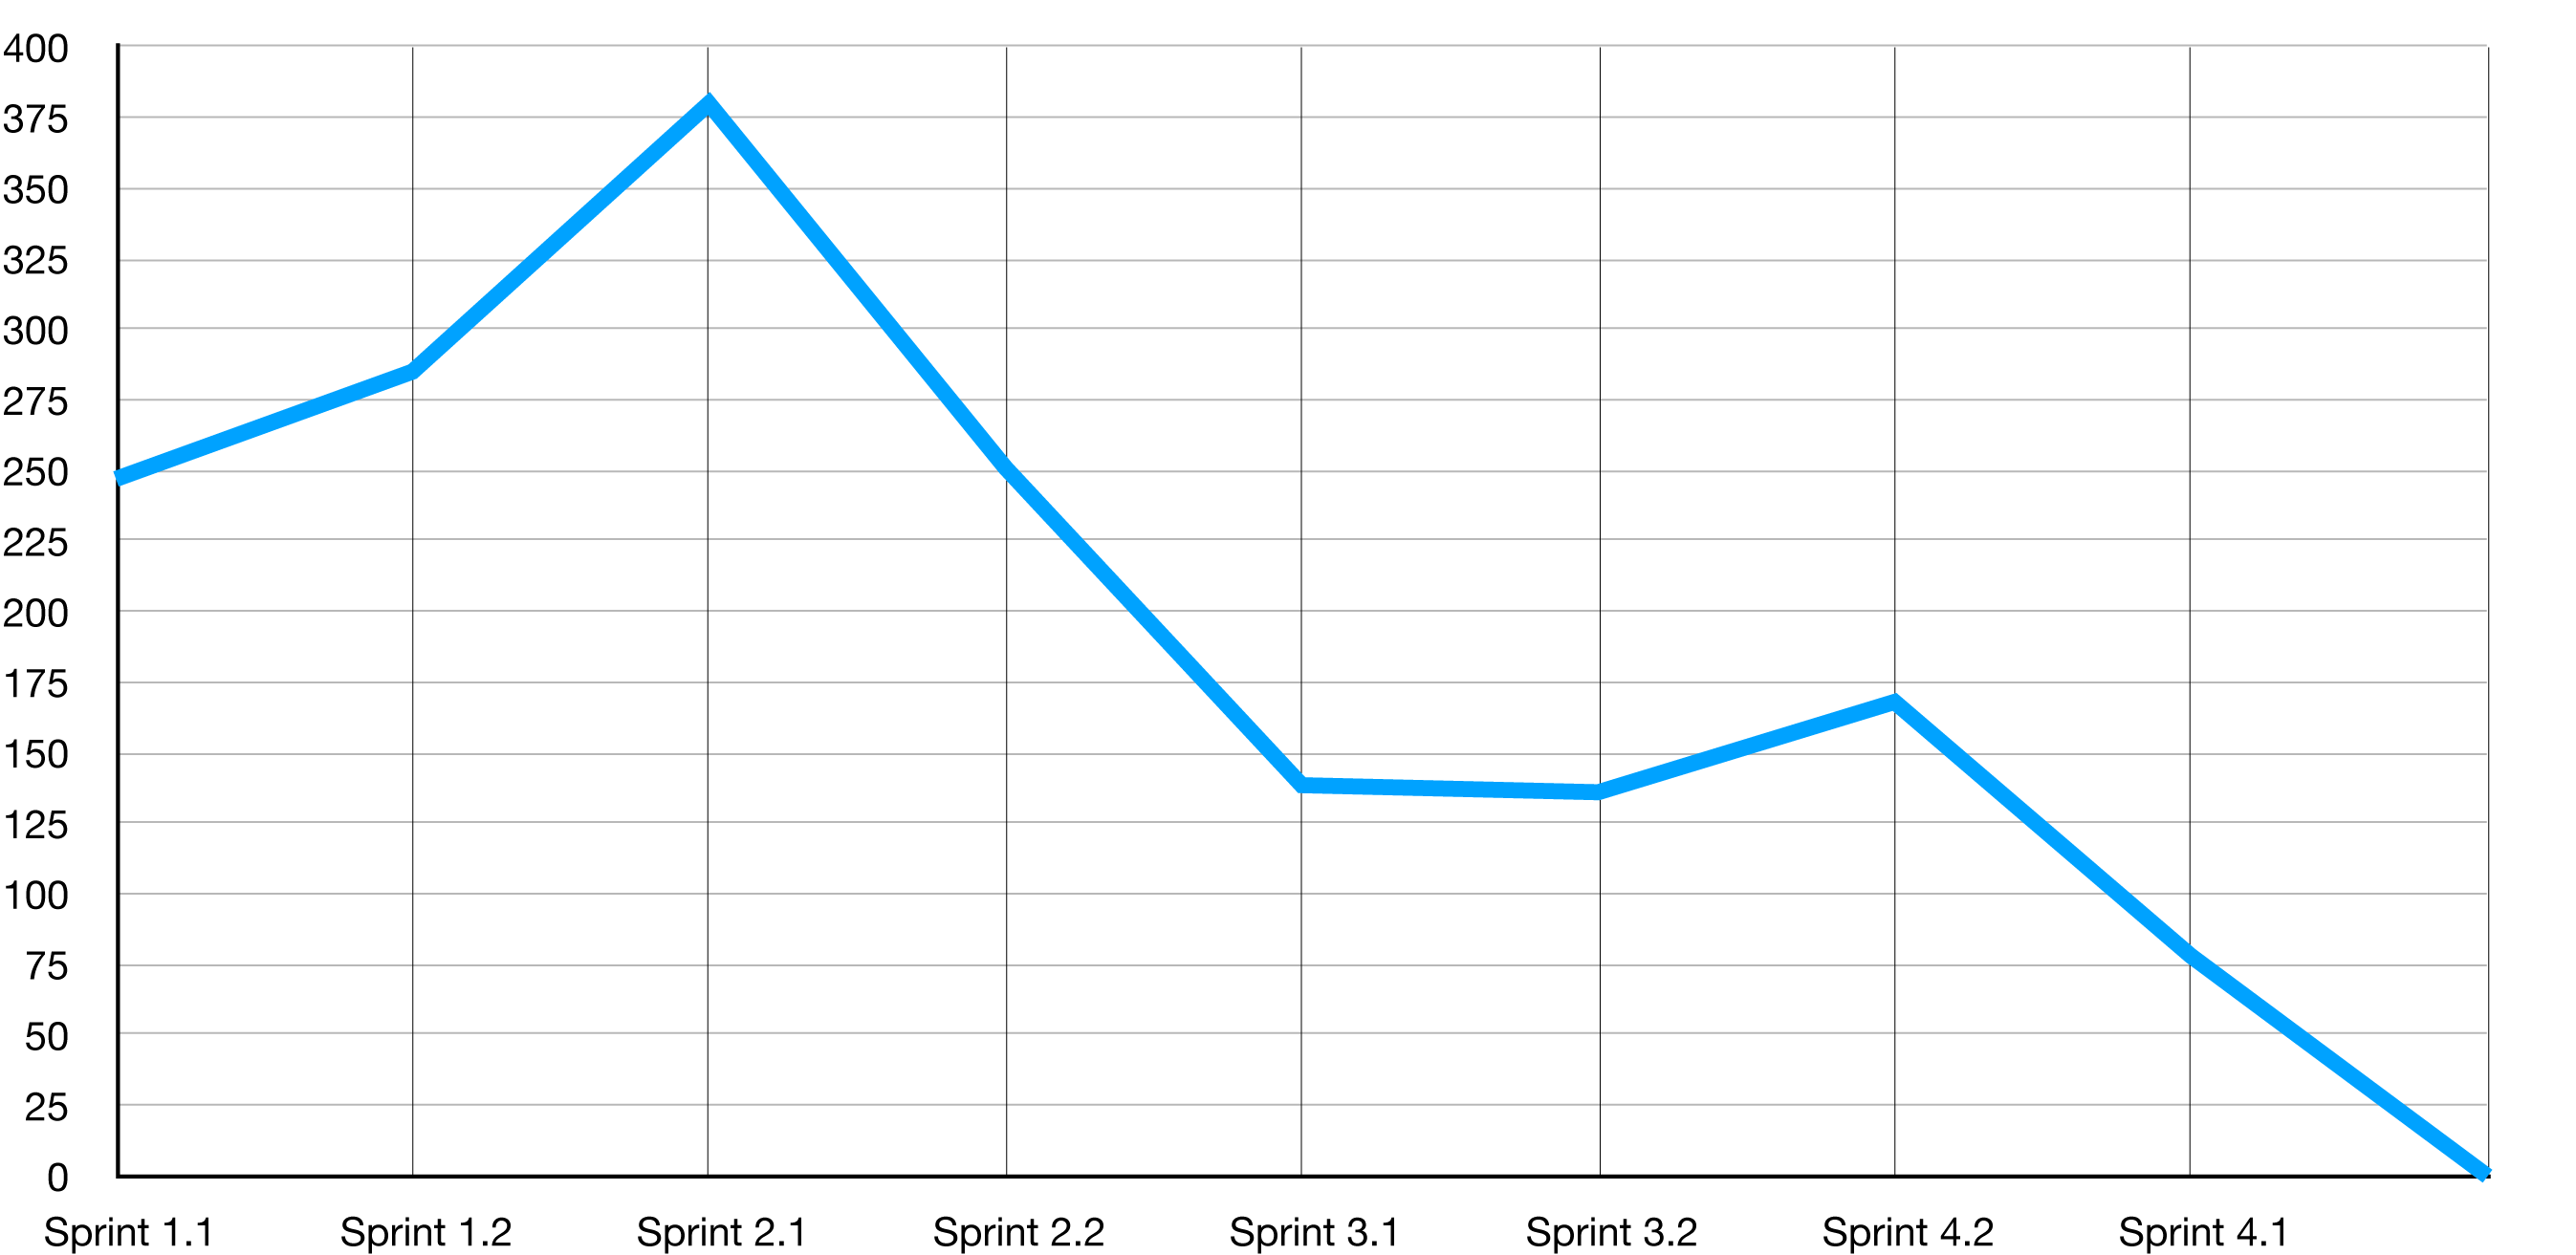
\includegraphics[width=11cm]{../burndown/burndown_slides.png}
      \end{tabular}
\end{frame}

\begin{frame}
\frametitle{Tecnologie utilizzate}
\begin{itemize}
  \item HTML, CSS
  \item Javascript
  \item Gocker
  \begin{itemize}
  \item NodeJs (lato server)
  \item MongoDB (per eventuali database)
\end{itemize}
\end{itemize}
Metodologia di sviluppo
  \begin{itemize}
  \item Scrum
\end{itemize}
      \centering  \begin{tabular}{c}
        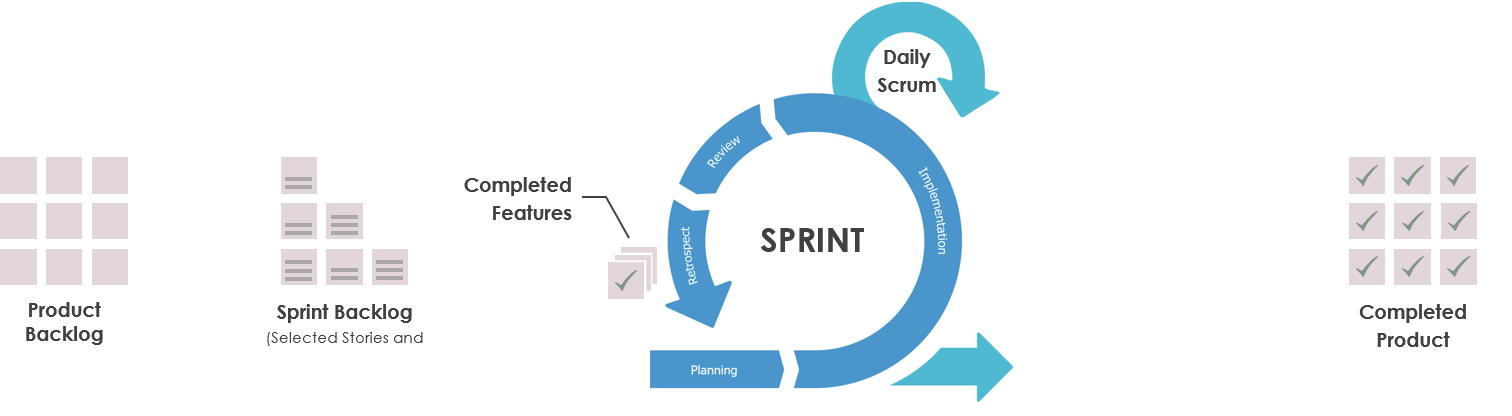
\includegraphics[width=11cm]{Images/scrum/scrum-sprint}
      \end{tabular}
\end{frame}

\begin{frame}
\frametitle{Software CAS}
\framesubtitle{GitLab}
GitLab è lo strumento di version control e repository utilizzato per il progetto.\\
Git ci ha permesso di scrivere codice evitando conflitti tra le varie copie/versioni dei sorgenti.
  \begin{itemize}
	\item Branch separati per sviluppo
  \end{itemize}
      \centering
        \begin{tabular}{c}
        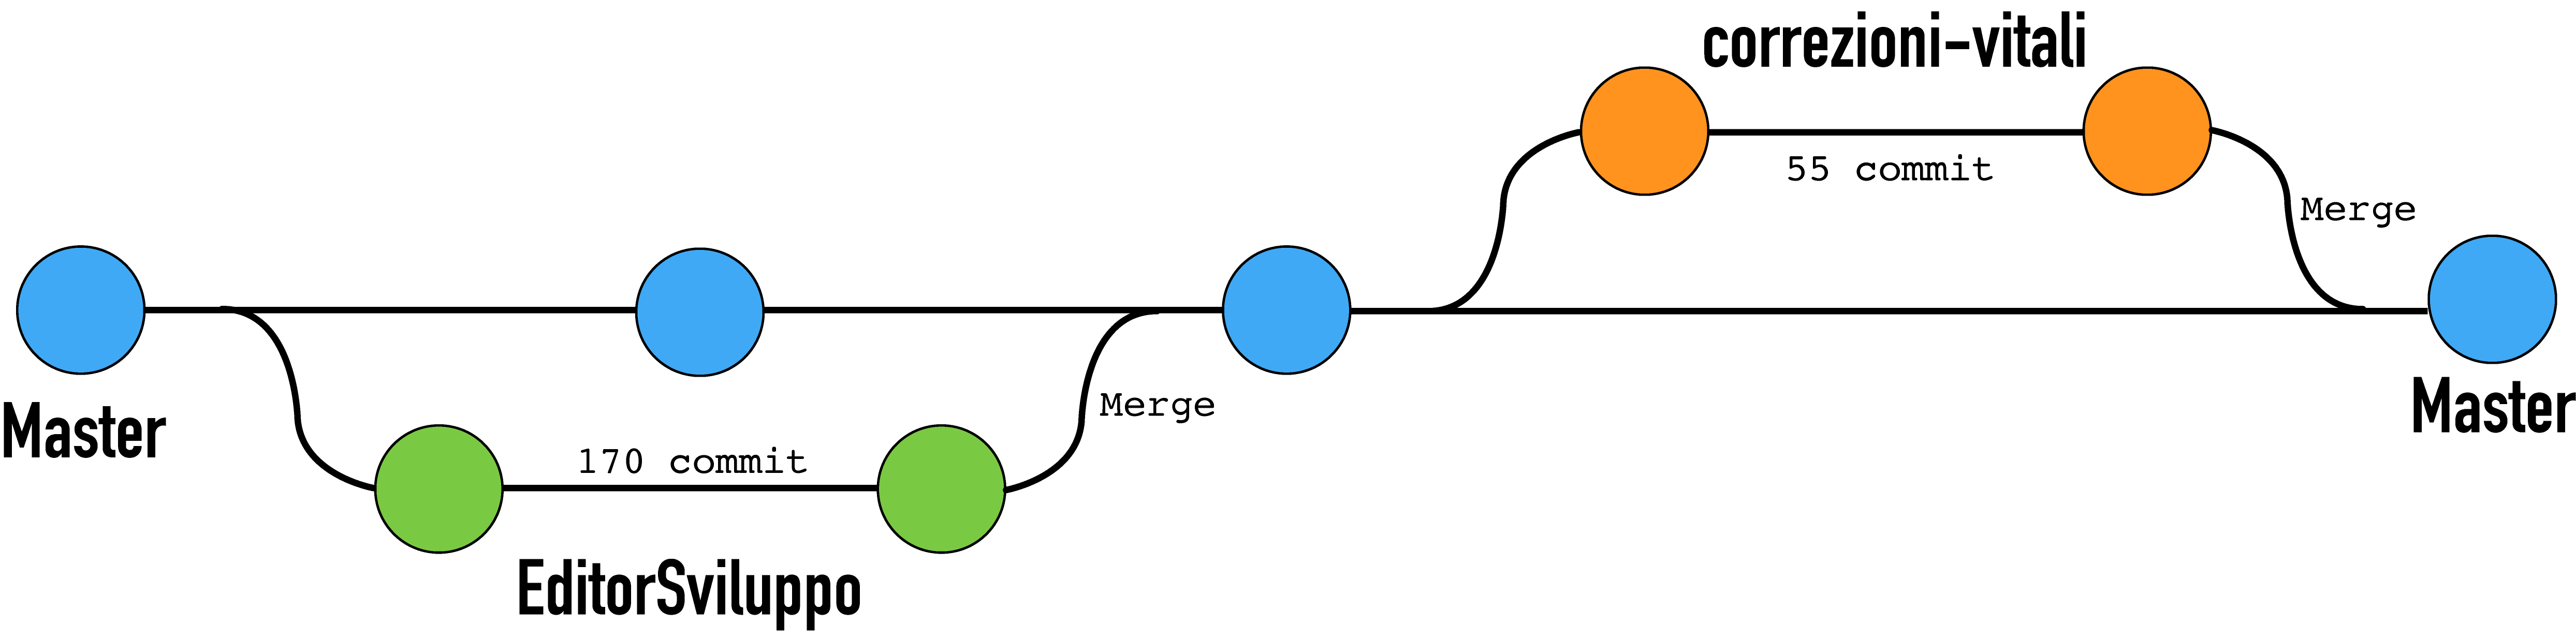
\includegraphics[width=11cm]{Images/GitLab/branches2}
      \end{tabular}
\end{frame}

\begin{frame}
\frametitle{Software CAS}
\framesubtitle{Mattermost}
MatterMost è la soluzione OpenSource per gestire le comunicazioni tra i membri di un gruppo di lavoro sia che si trovino negli stessi uffici sia che lavorino da remoto tramite telelavoro.\\
\vspace{0.2cm}
Noi in particolare abbiamo creato due canali di comunicazione diversi, con obbiettivi diversi:
\vspace{0.2cm}
\begin{columns}
\column{0.5\textwidth}
\centering
Idee
  \begin{itemize}
	\item Nuove
	\item In corso di sviluppo
	\item Scartate
	\item Finite
  \end{itemize}
\column{0.5\textwidth}
\centering
Bugs
  \begin{itemize}
	\item Nuovi
	\item Macchine di laboratorio
	\item HTML, CSS, JavaScript
	\item Risolti
  \end{itemize}
\end{columns}
\end{frame}

%\begin{frame}
%\frametitle{Software CAS}
%\framesubtitle{SonarQube}
%SonarQube è un’applicazione web che produce report sul codice duplicato, sugli standard di programmazione, i test di unità , il code coverage, la complessità , i bug potenziali, i commenti, la progettazione e l’architettura.
%  \begin{itemize}
%	\item Ogni bug segnalato è stato risolto
%	\item L'utilizzo di tecnologie deprecate sono state sostituite
%	\item Eventuali codici duplicati sono stati eliminati (in particolare CSS)
%	\item Commenti inutili sono stati cancellati
%  \end{itemize}
%\end{frame}

\begin{frame}
\frametitle{Software CAS}
\framesubtitle{Innometrics}
\begin{columns}
\column{0.5\textwidth}
Collector\\
Il collector monitora quanto tempo passiamo su ogni applicazione o sito web.
\column{0.5\textwidth}
Transfer\\
Innometrics Transfer permette di vedere i dati raccolti da Collector.\\
È possibile filtrare e/o caricare i dati su un server.
\end{columns}
\end{frame}

\begin{frame}
\frametitle{Impressioni personali}
\framesubtitle{Filippo Bartolucci}
Umberto puzza
\end{frame}

\begin{frame}
\frametitle{Impressioni personali}
\framesubtitle{Umberto Case}
Ho lavorato principalmente sulla parte browser del nostro progetto WhereMI, in coppia con Filippo.
Lascio alcune impressioni personali sui software utilizzati per realizzare il progetto:
\begin{itemize}
\item Taiga\\
Bella scoperta, lo ritengo un software indispensabile per organizzare il lavoro di gruppo.
Ci ha aiutato molto a dividere il lavoro e a focalizzarci su ogni user story in maniera definita.

\item Mattermost\\
Uno strumento utile per la chat del progetto, riportando solo informazioni rilevanti e privo di distrazioni esterne.
Abbiamo diviso la chat in due sezioni, una che riportava bug e problemi e l’altra relativa a idee per il progetto.
Lo ritengo utile ma non indispensabile.

\item GitLab\\
A differenza di Mattermost, questo strumento si è rivelato indispensabile per il lavoro di gruppo.
Diversi branch per diverse versioni del progetto.
Con tutte le commit eseguite, senza GitLab, sarebbe stato praticamente impossibile avere sempre il codice aggiornato e senza duplicati o contrasti.

\item SonarQube\\
Strumento che non conoscevo, è stato fondamentale per trovare bug e migliorare complessivamente il codice scritto.
 \end{itemize}
\end{frame}

\begin{frame}
\frametitle{Impressioni personali}
\framesubtitle{Francesco Cerio}
\begin{itemize}
	\item Taiga
	\item Gitlab	
	\item Sonarqube
	\item Mattermost
  \end{itemize}
\end{frame}

\begin{frame}
\frametitle{Impressioni personali}
\framesubtitle{Matteo Celani}
1/2 del "team Editor", ho lavorato a stretto contatto con Francesco. \\ Abbiamo svolto congiuntamente gli step finali del progetto aggregando le due parti.
\begin{columns}
	\column{0.5\textwidth}
  \begin{itemize}
	\item Taiga
		\begin{itemize}
			\item creazione sotto obiettivi	
			\item fondamentale per seguire sviluppo
 		 \end{itemize} 
	\item Gitlab 
		\begin{itemize}
			\item software più utilizzato	
			\item codice sempre aggiornato
			\item lavorato soprattutto su "Editor Sviluppo"
 		 \end{itemize}
  \end{itemize}
\column{0.5\textwidth}
\begin{itemize}
	\item Sonarqube 		
		\begin{itemize}
			\item corretti bug	
			\item evitate codice duplicato
			\item CSS efficace 
 		 \end{itemize}
	\item Mattermost 		\begin{itemize}
			\item usato sopratutto app mobile 	
			\item comunicato bug trovati
			\item comunicato evoluzioni del codice
 		 \end{itemize} 
	  \end{itemize}
\end{columns}
\end{frame}

\begin{frame}
\frametitle{Impressioni finali}
Abbiamo stilato una "classifica" in base a quanto ci sono stati utili i software utilizzati:
  \begin{enumerate}
	\item Taiga
	\item GitLab
	\item SonarQube
	\item Mattermost
  \end{enumerate}
  Software che non abbiamo ritenuto indispensabili:
  \begin{enumerate}
	\item Innometrics
  \end{enumerate}
\end{frame}

\begin{frame}
\frametitle{Impressioni finali}
I software utilizzati ci hanno aiutato parecchio nello sviluppo del codice, in particolare per organizzar le idee.\\
Taiga ci ha dato una grande mano a portare avanti un lavoro ben strutturato ed organizzato.\\
SonarQube è stato utile a trovare bug in modo facile e veloce ed a utilizzare tecniche di scrittura di codice più efficienti.\\
Mattermost è un canale di comunicazione completo, quindi siamo riusciti a comunicare in modo facile e veloce, inoltrando link e file senza avere problemi. Grazie all'applicazione mobile la comunicazione e la recezione dei messaggi è stata veloce.
Manca Git Lab
\end{frame}

\end{document}
